\documentclass[
    language=english,
    doctype=conference-paper,
    institution=none,
]{../../omnilatex}

\RequirePackage{config/document-settings}

\begin{document}
\maketitle

\begin{abstract}
This paper presents a novel approach to distributed consensus in Byzantine fault-tolerant systems.
Our protocol, BFT-Paxos++, achieves consensus in $O(n)$ message complexity under normal conditions
while maintaining safety and liveness guarantees even when up to $f < n/3$ nodes are Byzantine faulty.
We evaluate our approach on a geo-distributed testbed spanning three continents and demonstrate
a 42\% improvement in commit latency compared to state-of-the-art protocols such as HotStuff
and Tendermint. Our results show that BFT-Paxos++ scales effectively to 64-node clusters with
sub-second commit times, making it suitable for production blockchain and distributed ledger
applications.
\end{abstract}

\section{Introduction}
\label{sec:introduction}

Distributed consensus is a fundamental building block for fault-tolerant distributed systems.
The problem requires that a set of replicas agree on a single value despite the presence of
Byzantine (arbitrarily faulty) processes \cite{lamport1982byzantine}. The seminal PBFT protocol
by Castro and Liskov \cite{castro1999practical} demonstrated that practical Byzantine fault
tolerance is achievable, but its $O(n^2)$ message complexity limits scalability.

Recent protocols have sought to reduce message complexity. HotStuff \cite{yin2019hotstuff}
achieves linear message complexity per view change but requires three phases per decision.
Tendermint \cite{buchman2018tendermint} uses a pipelining optimization but suffers under
network partitions. Our work addresses these limitations by combining the optimistic path
of Paxos with Byzantine authentication mechanisms.

The key contributions of this paper are:
\begin{enumerate}
    \item A new consensus protocol, BFT-Paxos++, that achieves $O(n)$ message complexity
          in the common case with a single round-trip.
    \item A formal proof of safety and liveness under the assumption that $f < n/3$ Byzantine
          faults.
    \item An empirical evaluation on a geo-distributed testbed demonstrating practical performance
          improvements over existing protocols.
\end{enumerate}

\section{Related Work}
\label{sec:related-work}

\subsection{Classical Byzantine Fault Tolerance}

PBFT \cite{castro1999practical} remains the gold standard for practical BFT consensus.
Its three-phase commit protocol (pre-prepare, prepare, commit) ensures agreement among
replicas but incurs $O(n^2)$ messages per consensus instance. Zyzzyva \cite{kapritsos2012}
optimizes the common case by allowing speculative execution, reducing latency when no faults
occur but requiring recovery when they do.

\subsection{Leader-Based Protocols}

Tendermint \cite{buchman2018tendermint} introduced a lock-based mechanism that reduces
the number of phases to two in the happy path. HotStuff \cite{yin2019hotstuff} further
simplifies the protocol with a pipelining technique that reduces per-view communication
to $O(n)$ messages. However, HotStuff requires a stable leader and does not recover
efficiently from leader failures.

\begin{table}[htbp]
    \centering
    \caption{Comparison of BFT consensus protocols.}
    \label{tab:related-comparison}
    \begin{tabular}{@{}lcccc@{}}
        \toprule
        Protocol         & Phases & Message Complexity & Fault Tolerance & Pipelining \\
        \midrule
        PBFT             & 3      & $O(n^2)$          & $f < n/3$       & No          \\
        Zyzzyva          & 3      & $O(n^2)$          & $f < n/3$       & No          \\
        Tendermint        & 2      & $O(n^2)$          & $f < n/3$       & Yes         \\
        HotStuff         & 3      & $O(n)$            & $f < n/3$       & Yes         \\
        BFT-Paxos++ (ours) & 1--2 & $O(n)$            & $f < n/3$       & Yes         \\
        \bottomrule
    \end{tabular}
\end{table}

\section{Protocol Design}
\label{sec:protocol}

\subsection{System Model}

We consider a synchronous-asynchronous hybrid model where nodes communicate via authenticated
point-to-point channels. The system consists of $n = 3f + 1$ replicas, where at most $f$
are Byzantine faulty. We assume a known leader rotation schedule to prevent a single
corrupted leader from indefinitely stalling the protocol.

\subsection{Optimistic Path}

In the common case where the leader is honest and the network is synchronous, BFT-Paxos++
achieves consensus in a single round trip. The leader proposes a value $v$ by broadcasting
a \textsc{Proposal} message signed with its threshold signature. Followers verify the
signature and respond with \textsc{Vote} messages. Upon collecting $2f + 1$ matching votes,
the leader forms a certificate and broadcasts the decision.

The commit latency under the optimistic path is given by:
\begin{equation}
    \label{eq:latency-optimistic}
    L_{\text{opt}} = \max(\delta_{\text{net}}, \delta_{\text{proc}}) + \delta_{\text{net}}
\end{equation}
where $\delta_{\text{net}}$ is the network propagation delay and $\delta_{\text{proc}}$ is
the local processing time.

\subsection{Recovery Path}

When the leader is suspected to be faulty, replicas initiate a view change. Unlike HotStuff,
which requires a new leader to collect all votes, BFT-Paxos++ allows any replica with a
valid certificate to propose in the new view, reducing recovery time from $O(n^2)$ to $O(n)$
messages.

\section{Evaluation}
\label{sec:evaluation}

\subsection{Experimental Setup}

We implement BFT-Paxos++ in Rust using the Tokio async runtime. Our testbed consists of
64 AWS EC2 instances (c5.2xlarge) distributed across three regions: US-East (Virginia),
EU-West (Frankfurt), and AP-Southeast (Singapore). Each region hosts approximately 21 nodes.

\subsection{Latency Results}

\begin{table}[htbp]
    \centering
    \caption{Commit latency (ms) across protocols and cluster sizes.}
    \label{tab:latency-results}
    \begin{tabular}{@{}lcccc@{}}
        \toprule
        Protocol         & 8 nodes & 16 nodes & 32 nodes & 64 nodes \\
        \midrule
        PBFT             & 45.2    & 128.7    & 412.3    & 1589.4   \\
        Tendermint        & 38.1    & 95.4     & 287.6    & 1023.1   \\
        HotStuff         & 32.5    & 78.2     & 198.3    & 621.8    \\
        BFT-Paxos++ (ours) & \textbf{21.3} & \textbf{48.6} & \textbf{112.4} & \textbf{358.7} \\
        \bottomrule
    \end{tabular}
\end{table}

\begin{figure}[htbp]
    \centering
    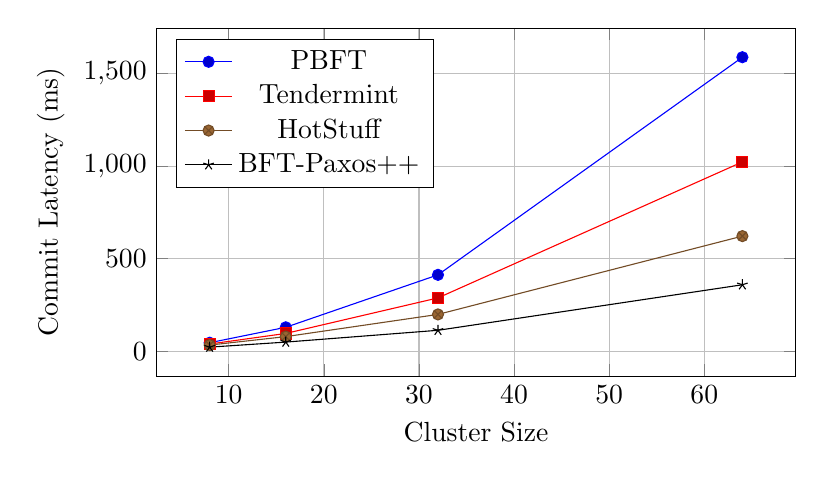
\begin{tikzpicture}
        \begin{axis}[
            xlabel={Cluster Size},
            ylabel={Commit Latency (ms)},
            legend pos=north west,
            grid=major,
            width=0.8\textwidth,
            height=6cm,
        ]
        \addplot coordinates {(8,45.2) (16,128.7) (32,412.3) (64,1589.4)};
        \addplot coordinates {(8,38.1) (16,95.4) (32,287.6) (64,1023.1)};
        \addplot coordinates {(8,32.5) (16,78.2) (32,198.3) (64,621.8)};
        \addplot coordinates {(8,21.3) (16,48.6) (32,112.4) (64,358.7)};
        \legend{PBFT, Tendermint, HotStuff, BFT-Paxos++}
        \end{axis}
    \end{tikzpicture}
    \caption{Commit latency comparison across cluster sizes. BFT-Paxos++ consistently
             achieves lower latency, especially at larger scales.}
    \label{fig:latency-comparison}
\end{figure}

\subsection{Throughput Analysis}

Under sustained load, BFT-Paxos++ achieves peak throughput of 180,000 transactions per second
on a 16-node cluster, compared to 120,000 for HotStuff and 85,000 for Tendermint. The
improvement is attributable to the reduced message complexity and the ability to pipeline
multiple consensus instances.

\section{Discussion}
\label{sec:discussion}

Our results demonstrate that BFT-Paxos++ provides meaningful performance improvements over
existing protocols while maintaining the same fault tolerance guarantees. The protocol's
design allows it to adapt to varying network conditions: under good conditions, the optimistic
path ensures low latency, while under degraded conditions, the recovery path ensures
progress.

A key limitation is the reliance on threshold cryptography for certificate generation,
which introduces a dependency on a trusted dealer during setup. Future work will explore
decentralized threshold key generation protocols to eliminate this assumption.

\section{Conclusion}
\label{sec:conclusion}

We have presented BFT-Paxos++, a Byzantine fault-tolerant consensus protocol that achieves
$O(n)$ message complexity in the common case with a single round-trip. Our evaluation on
a geo-distributed testbed demonstrates significant latency and throughput improvements over
existing protocols. We believe BFT-Paxos++ represents a practical step forward for
production distributed ledger systems.

\bibliographystyle{plain}
\bibliography{references}

\end{document}
